\tikzset {_cuejj3ut6/.code = {\pgfsetadditionalshadetransform{ \pgftransformshift{\pgfpoint{0 bp } { 0 bp }  }  \pgftransformrotate{-117 }  \pgftransformscale{2 }  }}}
\pgfdeclarehorizontalshading{_5ugpqis72}{150bp}{rgb(0bp)=(1,1,1);
    rgb(37.5bp)=(1,1,1);
    rgb(50.08184160505022bp)=(0.95,0.95,0.95);
    rgb(57.64583042689732bp)=(0.88,0.88,0.88);
    rgb(61.33184160505022bp)=(0.96,0.96,0.96);
    rgb(100bp)=(0.96,0.96,0.96)}
\tikzset {_d6bvf3ads/.code = {\pgfsetadditionalshadetransform{ \pgftransformshift{\pgfpoint{0 bp } { 0 bp }  }  \pgftransformrotate{-117 }  \pgftransformscale{2 }  }}}
\pgfdeclarehorizontalshading{_xx64avkmf}{150bp}{rgb(0bp)=(1,1,1);
    rgb(37.5bp)=(1,1,1);
    rgb(50.08184160505022bp)=(0.95,0.95,0.95);
    rgb(57.64583042689732bp)=(0.88,0.88,0.88);
    rgb(61.33184160505022bp)=(0.96,0.96,0.96);
    rgb(100bp)=(0.96,0.96,0.96)}
\tikzset {_gxyzl2ql8/.code = {\pgfsetadditionalshadetransform{ \pgftransformshift{\pgfpoint{0 bp } { 0 bp }  }  \pgftransformrotate{-117 }  \pgftransformscale{2 }  }}}
\pgfdeclarehorizontalshading{_Aokbkkxvx}{150bp}{rgb(0bp)=(1,1,1);
    rgb(37.5bp)=(1,1,1);
    rgb(50.08184160505022bp)=(0.95,0.95,0.95);
    rgb(57.64583042689732bp)=(0.88,0.88,0.88);
    rgb(61.33184160505022bp)=(0.96,0.96,0.96);
    rgb(100bp)=(0.96,0.96,0.96)}
\tikzset {_m8uplal2o/.code = {\pgfsetadditionalshadetransform{ \pgftransformshift{\pgfpoint{0 bp } { 0 bp }  }  \pgftransformrotate{-117 }  \pgftransformscale{2 }  }}}
\pgfdeclarehorizontalshading{_i8uv4t2gq}{150bp}{rgb(0bp)=(1,1,1);
    rgb(37.5bp)=(1,1,1);
    rgb(50.08184160505022bp)=(0.95,0.95,0.95);
    rgb(57.64583042689732bp)=(0.88,0.88,0.88);
    rgb(61.33184160505022bp)=(0.96,0.96,0.96);
    rgb(100bp)=(0.96,0.96,0.96)}
\tikzset {_60x67noot/.code = {\pgfsetadditionalshadetransform{ \pgftransformshift{\pgfpoint{0 bp } { 0 bp }  }  \pgftransformrotate{-117 }  \pgftransformscale{2 }  }}}
\pgfdeclarehorizontalshading{_wjk5bthop}{150bp}{rgb(0bp)=(1,1,1);
    rgb(37.5bp)=(1,1,1);
    rgb(50.08184160505022bp)=(0.95,0.95,0.95);
    rgb(57.64583042689732bp)=(0.88,0.88,0.88);
    rgb(61.33184160505022bp)=(0.96,0.96,0.96);
    rgb(100bp)=(0.96,0.96,0.96)}
\tikzset {_cf91rnvay/.code = {\pgfsetadditionalshadetransform{ \pgftransformshift{\pgfpoint{0 bp } { 0 bp }  }  \pgftransformrotate{-117 }  \pgftransformscale{2 }  }}}
\pgfdeclarehorizontalshading{_e8wxk8n2i}{150bp}{rgb(0bp)=(1,1,1);
    rgb(37.5bp)=(1,1,1);
    rgb(50.08184160505022bp)=(0.95,0.95,0.95);
    rgb(57.64583042689732bp)=(0.88,0.88,0.88);
    rgb(61.33184160505022bp)=(0.96,0.96,0.96);
    rgb(100bp)=(0.96,0.96,0.96)}
\tikzset{every picture/.style={line width=0.75pt}}
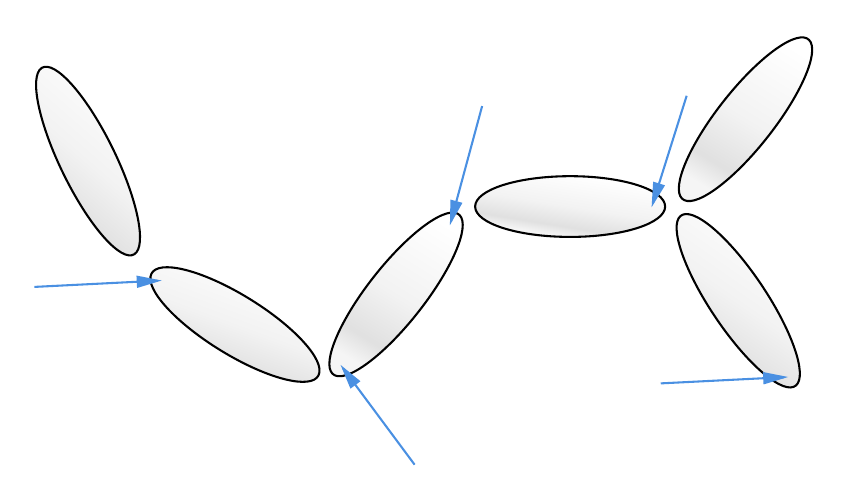
\begin{tikzpicture}[x=0.75pt,y=0.75pt,yscale=-1,xscale=1]
    \path  [shading=_5ugpqis72,_cuejj3ut6] (324.59,122.77) .. controls (324.59,114.69) and (345.08,108.14) .. (370.37,108.14) .. controls (395.65,108.14) and (416.14,114.69) .. (416.14,122.77) .. controls (416.14,130.85) and (395.65,137.4) .. (370.37,137.4) .. controls (345.08,137.4) and (324.59,130.85) .. (324.59,122.77) -- cycle ;
    \draw  [color={rgb, 255:red, 0; green, 0; blue, 0 }  ,draw opacity=1 ][line width=0.75]  (324.59,122.77) .. controls (324.59,114.69) and (345.08,108.14) .. (370.37,108.14) .. controls (395.65,108.14) and (416.14,114.69) .. (416.14,122.77) .. controls (416.14,130.85) and (395.65,137.4) .. (370.37,137.4) .. controls (345.08,137.4) and (324.59,130.85) .. (324.59,122.77) -- cycle ;
    \path  [shading=_xx64avkmf,_d6bvf3ads] (485.49,42.5) .. controls (490.83,47.9) and (481.46,69.38) .. (464.54,90.48) .. controls (447.63,111.58) and (429.58,124.31) .. (424.23,118.9) .. controls (418.88,113.5) and (428.26,92.02) .. (445.18,70.92) .. controls (462.09,49.82) and (480.14,37.09) .. (485.49,42.5) -- cycle ;
    \draw  [color={rgb, 255:red, 0; green, 0; blue, 0 }  ,draw opacity=1 ][line width=0.75]  (485.49,42.5) .. controls (490.83,47.9) and (481.46,69.38) .. (464.54,90.48) .. controls (447.63,111.58) and (429.58,124.31) .. (424.23,118.9) .. controls (418.88,113.5) and (428.26,92.02) .. (445.18,70.92) .. controls (462.09,49.82) and (480.14,37.09) .. (485.49,42.5) -- cycle ;
    \path  [shading=_Aokbkkxvx,_gxyzl2ql8] (317.12,126.9) .. controls (322.47,132.3) and (313.09,153.79) .. (296.17,174.89) .. controls (279.26,195.98) and (261.21,208.71) .. (255.86,203.31) .. controls (250.52,197.9) and (259.89,176.42) .. (276.81,155.32) .. controls (293.72,134.22) and (311.77,121.5) .. (317.12,126.9) -- cycle ;
    \draw  [color={rgb, 255:red, 0; green, 0; blue, 0 }  ,draw opacity=1 ][line width=0.75]  (317.12,126.9) .. controls (322.47,132.3) and (313.09,153.79) .. (296.17,174.89) .. controls (279.26,195.98) and (261.21,208.71) .. (255.86,203.31) .. controls (250.52,197.9) and (259.89,176.42) .. (276.81,155.32) .. controls (293.72,134.22) and (311.77,121.5) .. (317.12,126.9) -- cycle ;
    \path  [shading=_i8uv4t2gq,_m8uplal2o] (160.4,145.75) .. controls (154.11,149.69) and (139.04,132.78) .. (126.72,107.99) .. controls (114.4,83.2) and (109.51,59.91) .. (115.79,55.97) .. controls (122.07,52.03) and (137.15,68.94) .. (149.47,93.73) .. controls (161.79,118.53) and (166.68,141.82) .. (160.4,145.75) -- cycle ;
    \draw  [color={rgb, 255:red, 0; green, 0; blue, 0 }  ,draw opacity=1 ][line width=0.75]  (160.4,145.75) .. controls (154.11,149.69) and (139.04,132.78) .. (126.72,107.99) .. controls (114.4,83.2) and (109.51,59.91) .. (115.79,55.97) .. controls (122.07,52.03) and (137.15,68.94) .. (149.47,93.73) .. controls (161.79,118.53) and (166.68,141.82) .. (160.4,145.75) -- cycle ;
    \path  [shading=_wjk5bthop,_60x67noot] (168.6,155.19) .. controls (172.02,148.08) and (192.82,153.25) .. (215.07,166.74) .. controls (237.32,180.23) and (252.58,196.93) .. (249.16,204.04) .. controls (245.74,211.15) and (224.93,205.98) .. (202.69,192.49) .. controls (180.44,179) and (165.18,162.3) .. (168.6,155.19) -- cycle ;
    \draw  [color={rgb, 255:red, 0; green, 0; blue, 0 }  ,draw opacity=1 ][line width=0.75]  (168.6,155.19) .. controls (172.02,148.08) and (192.82,153.25) .. (215.07,166.74) .. controls (237.32,180.23) and (252.58,196.93) .. (249.16,204.04) .. controls (245.74,211.15) and (224.93,205.98) .. (202.69,192.49) .. controls (180.44,179) and (165.18,162.3) .. (168.6,155.19) -- cycle ;
    \path  [shading=_e8wxk8n2i,_cf91rnvay] (479.18,208.97) .. controls (473.47,213.88) and (456.38,199.59) .. (441,177.05) .. controls (425.63,154.51) and (417.81,132.26) .. (423.52,127.34) .. controls (429.23,122.43) and (446.32,136.72) .. (461.69,159.26) .. controls (477.07,181.8) and (484.89,204.06) .. (479.18,208.97) -- cycle ;
    \draw  [color={rgb, 255:red, 0; green, 0; blue, 0 }  ,draw opacity=1 ][line width=0.75]  (479.18,208.97) .. controls (473.47,213.88) and (456.38,199.59) .. (441,177.05) .. controls (425.63,154.51) and (417.81,132.26) .. (423.52,127.34) .. controls (429.23,122.43) and (446.32,136.72) .. (461.69,159.26) .. controls (477.07,181.8) and (484.89,204.06) .. (479.18,208.97) -- cycle ;
    \draw [color={rgb, 255:red, 74; green, 144; blue, 226 }  ,draw opacity=1 ]   (112.21,161.49) -- (171.56,158.51) ;
    \draw [shift={(173.55,158.41)}, rotate = 177.12] [fill={rgb, 255:red, 74; green, 144; blue, 226 }  ,fill opacity=1 ][line width=0.08]  [draw opacity=0] (12,-3) -- (0,0) -- (12,3) -- cycle    ;
    \draw [color={rgb, 255:red, 74; green, 144; blue, 226 }  ,draw opacity=1 ]   (327.97,74.35) -- (312.97,129.84) ;
    \draw [shift={(312.45,131.77)}, rotate = 285.13] [fill={rgb, 255:red, 74; green, 144; blue, 226 }  ,fill opacity=1 ][line width=0.08]  [draw opacity=0] (12,-3) -- (0,0) -- (12,3) -- cycle    ;
    \draw [color={rgb, 255:red, 74; green, 144; blue, 226 }  ,draw opacity=1 ]   (414.02,207.97) -- (473.37,204.99) ;
    \draw [shift={(475.37,204.89)}, rotate = 177.12] [fill={rgb, 255:red, 74; green, 144; blue, 226 }  ,fill opacity=1 ][line width=0.08]  [draw opacity=0] (12,-3) -- (0,0) -- (12,3) -- cycle    ;
    \draw [color={rgb, 255:red, 74; green, 144; blue, 226 }  ,draw opacity=1 ]   (426.51,69.4) -- (410.22,121.19) ;
    \draw [shift={(409.62,123.1)}, rotate = 287.47] [fill={rgb, 255:red, 74; green, 144; blue, 226 }  ,fill opacity=1 ][line width=0.08]  [draw opacity=0] (12,-3) -- (0,0) -- (12,3) -- cycle    ;
    \draw [color={rgb, 255:red, 74; green, 144; blue, 226 }  ,draw opacity=1 ]   (295.44,247.14) -- (260.97,200.71) ;
    \draw [shift={(259.78,199.1)}, rotate = 53.41] [fill={rgb, 255:red, 74; green, 144; blue, 226 }  ,fill opacity=1 ][line width=0.08]  [draw opacity=0] (12,-3) -- (0,0) -- (12,3) -- cycle    ;
\end{tikzpicture}